\documentclass[14pt,fleqn]{extarticle}

\usepackage[french]{babel}
\usepackage[utf8]{inputenc}
\usepackage[T1]{fontenc}

\usepackage{amsmath,amssymb,amsthm}
\usepackage{graphicx}

\usepackage{pstricks,pst-plot,pst-tree,pstricks-add}
\usepackage{pst-eucl}
\usepackage{pst-node}
\usepackage{enumitem}
\usepackage{hyperref}

\usepackage{geometry}
\geometry{a4paper,total={190mm,257mm}}
\usepackage{fancyhdr}
	\pagestyle{plain} 
	\fancyfoot[C]{} 
	\fancyhead[L]{Nom, prénom : }
	\fancyhead[R]{}
	
	
	\title{Contrôle trigonométrie-fonctions affines}
	\date{}
	\begin{document} 

\subsection*{Exercice 1 (6 points)}
Pour chacune des fonctions suivantes dire si elle est linéaire, affine, ou aucun des deux, et donner son coefficient directeur et son ordonnée à l'origine lorsqu'elle est affine.
\begin{enumerate}
\item $f(x) = 2x+3$
\item $g(x) = \frac{-3x}{2}$
\item $h(x) = x^2 +(x-1)(x-2)$
\item $k(x) = (2x-1)(2x+2)-(x+5)(4x-1)$
\end{enumerate}

\subsection*{Exercice 2 (8 points)}

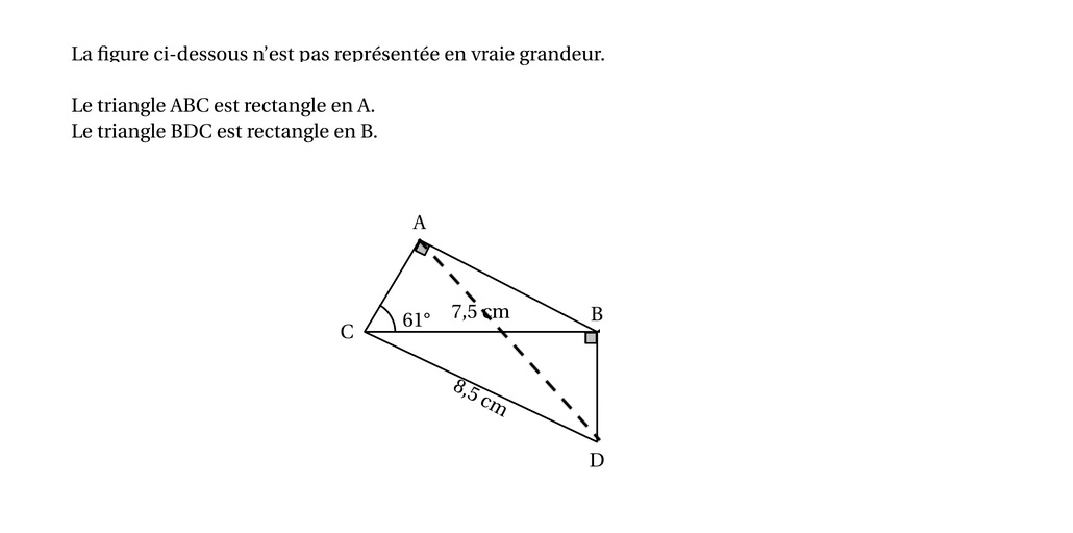
\includegraphics[scale=1]{Exo3.eps}
\begin{enumerate}
\item Calculer la longueur $AB$. 
\item Calculer l'angle $\widehat{BCD}$. 
\item Peut-on affirmer que $ACD$ est un triangle rectangle ?
\item Calculer l'aire du triangle $ABC$. 
\end{enumerate}


\subsection*{Exercice 4 ( 6 points)}
On considère la fonction $g$ tracée sur le repère-ci contre.\\
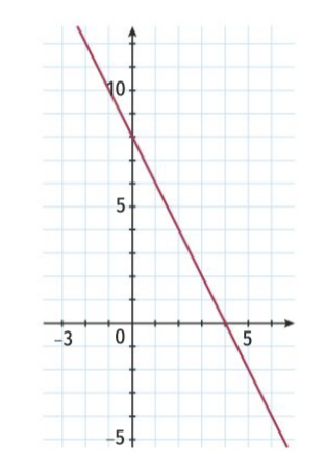
\includegraphics[scale=1.5]{Exo5.eps}
\\
On définit la fonction $f$ d'expression $f(x)=2x$. 
\begin{enumerate}
\item Quelle est la nature de la fonction $f$ ? 
\item Quelle est la nature de la fonction $g$ ? 
\item Tracer la courbe représentative de $f$ sur le repère. 
\item Déterminer l'expression de la fonction $g$ à partir du graphique. 
\item Donner les coordonnées du point d'intersection des droites représentatives de $f$ et $g$. 
\item Résoudre l'équation $f(x)=g(x)$ et commenter le résultat obtenu.
\end{enumerate}
\subsection*{Bonus}

Montrer que l'expression suivante définit une fonction affine dont on donnera la forme simplifiée : 
\[ (x-1)(x+2)(x-2) - (x-4)(x-2)(x+5)\]

 
 	\end{document}
 




